% Options for packages loaded elsewhere
\PassOptionsToPackage{unicode}{hyperref}
\PassOptionsToPackage{hyphens}{url}
%
\documentclass[
]{report}
\usepackage{amsmath,amssymb}
\usepackage{iftex}
\ifPDFTeX
  \usepackage[T1]{fontenc}
  \usepackage[utf8]{inputenc}
  \usepackage{textcomp} % provide euro and other symbols
\else % if luatex or xetex
  \usepackage{unicode-math} % this also loads fontspec
  \defaultfontfeatures{Scale=MatchLowercase}
  \defaultfontfeatures[\rmfamily]{Ligatures=TeX,Scale=1}
\fi
\usepackage{lmodern}
\ifPDFTeX\else
  % xetex/luatex font selection
\fi
% Use upquote if available, for straight quotes in verbatim environments
\IfFileExists{upquote.sty}{\usepackage{upquote}}{}
\IfFileExists{microtype.sty}{% use microtype if available
  \usepackage[]{microtype}
  \UseMicrotypeSet[protrusion]{basicmath} % disable protrusion for tt fonts
}{}
\makeatletter
\@ifundefined{KOMAClassName}{% if non-KOMA class
  \IfFileExists{parskip.sty}{%
    \usepackage{parskip}
  }{% else
    \setlength{\parindent}{0pt}
    \setlength{\parskip}{6pt plus 2pt minus 1pt}}
}{% if KOMA class
  \KOMAoptions{parskip=half}}
\makeatother
\usepackage{xcolor}
\usepackage{color}
\usepackage{fancyvrb}
\newcommand{\VerbBar}{|}
\newcommand{\VERB}{\Verb[commandchars=\\\{\}]}
\DefineVerbatimEnvironment{Highlighting}{Verbatim}{commandchars=\\\{\}}
% Add ',fontsize=\small' for more characters per line
\usepackage{framed}
\definecolor{shadecolor}{RGB}{248,248,248}
\newenvironment{Shaded}{\begin{snugshade}}{\end{snugshade}}
\newcommand{\AlertTok}[1]{\textcolor[rgb]{0.94,0.16,0.16}{#1}}
\newcommand{\AnnotationTok}[1]{\textcolor[rgb]{0.56,0.35,0.01}{\textbf{\textit{#1}}}}
\newcommand{\AttributeTok}[1]{\textcolor[rgb]{0.13,0.29,0.53}{#1}}
\newcommand{\BaseNTok}[1]{\textcolor[rgb]{0.00,0.00,0.81}{#1}}
\newcommand{\BuiltInTok}[1]{#1}
\newcommand{\CharTok}[1]{\textcolor[rgb]{0.31,0.60,0.02}{#1}}
\newcommand{\CommentTok}[1]{\textcolor[rgb]{0.56,0.35,0.01}{\textit{#1}}}
\newcommand{\CommentVarTok}[1]{\textcolor[rgb]{0.56,0.35,0.01}{\textbf{\textit{#1}}}}
\newcommand{\ConstantTok}[1]{\textcolor[rgb]{0.56,0.35,0.01}{#1}}
\newcommand{\ControlFlowTok}[1]{\textcolor[rgb]{0.13,0.29,0.53}{\textbf{#1}}}
\newcommand{\DataTypeTok}[1]{\textcolor[rgb]{0.13,0.29,0.53}{#1}}
\newcommand{\DecValTok}[1]{\textcolor[rgb]{0.00,0.00,0.81}{#1}}
\newcommand{\DocumentationTok}[1]{\textcolor[rgb]{0.56,0.35,0.01}{\textbf{\textit{#1}}}}
\newcommand{\ErrorTok}[1]{\textcolor[rgb]{0.64,0.00,0.00}{\textbf{#1}}}
\newcommand{\ExtensionTok}[1]{#1}
\newcommand{\FloatTok}[1]{\textcolor[rgb]{0.00,0.00,0.81}{#1}}
\newcommand{\FunctionTok}[1]{\textcolor[rgb]{0.13,0.29,0.53}{\textbf{#1}}}
\newcommand{\ImportTok}[1]{#1}
\newcommand{\InformationTok}[1]{\textcolor[rgb]{0.56,0.35,0.01}{\textbf{\textit{#1}}}}
\newcommand{\KeywordTok}[1]{\textcolor[rgb]{0.13,0.29,0.53}{\textbf{#1}}}
\newcommand{\NormalTok}[1]{#1}
\newcommand{\OperatorTok}[1]{\textcolor[rgb]{0.81,0.36,0.00}{\textbf{#1}}}
\newcommand{\OtherTok}[1]{\textcolor[rgb]{0.56,0.35,0.01}{#1}}
\newcommand{\PreprocessorTok}[1]{\textcolor[rgb]{0.56,0.35,0.01}{\textit{#1}}}
\newcommand{\RegionMarkerTok}[1]{#1}
\newcommand{\SpecialCharTok}[1]{\textcolor[rgb]{0.81,0.36,0.00}{\textbf{#1}}}
\newcommand{\SpecialStringTok}[1]{\textcolor[rgb]{0.31,0.60,0.02}{#1}}
\newcommand{\StringTok}[1]{\textcolor[rgb]{0.31,0.60,0.02}{#1}}
\newcommand{\VariableTok}[1]{\textcolor[rgb]{0.00,0.00,0.00}{#1}}
\newcommand{\VerbatimStringTok}[1]{\textcolor[rgb]{0.31,0.60,0.02}{#1}}
\newcommand{\WarningTok}[1]{\textcolor[rgb]{0.56,0.35,0.01}{\textbf{\textit{#1}}}}
\usepackage{longtable,booktabs,array}
\usepackage{calc} % for calculating minipage widths
% Correct order of tables after \paragraph or \subparagraph
\usepackage{etoolbox}
\makeatletter
\patchcmd\longtable{\par}{\if@noskipsec\mbox{}\fi\par}{}{}
\makeatother
% Allow footnotes in longtable head/foot
\IfFileExists{footnotehyper.sty}{\usepackage{footnotehyper}}{\usepackage{footnote}}
\makesavenoteenv{longtable}
\usepackage{graphicx}
\makeatletter
\def\maxwidth{\ifdim\Gin@nat@width>\linewidth\linewidth\else\Gin@nat@width\fi}
\def\maxheight{\ifdim\Gin@nat@height>\textheight\textheight\else\Gin@nat@height\fi}
\makeatother
% Scale images if necessary, so that they will not overflow the page
% margins by default, and it is still possible to overwrite the defaults
% using explicit options in \includegraphics[width, height, ...]{}
\setkeys{Gin}{width=\maxwidth,height=\maxheight,keepaspectratio}
% Set default figure placement to htbp
\makeatletter
\def\fps@figure{htbp}
\makeatother
\setlength{\emergencystretch}{3em} % prevent overfull lines
\providecommand{\tightlist}{%
  \setlength{\itemsep}{0pt}\setlength{\parskip}{0pt}}
\setcounter{secnumdepth}{5}
% definitions for citeproc citations
\NewDocumentCommand\citeproctext{}{}
\NewDocumentCommand\citeproc{mm}{%
  \begingroup\def\citeproctext{#2}\cite{#1}\endgroup}
\makeatletter
 % allow citations to break across lines
 \let\@cite@ofmt\@firstofone
 % avoid brackets around text for \cite:
 \def\@biblabel#1{}
 \def\@cite#1#2{{#1\if@tempswa , #2\fi}}
\makeatother
\newlength{\cslhangindent}
\setlength{\cslhangindent}{1.5em}
\newlength{\csllabelwidth}
\setlength{\csllabelwidth}{3em}
\newenvironment{CSLReferences}[2] % #1 hanging-indent, #2 entry-spacing
 {\begin{list}{}{%
  \setlength{\itemindent}{0pt}
  \setlength{\leftmargin}{0pt}
  \setlength{\parsep}{0pt}
  % turn on hanging indent if param 1 is 1
  \ifodd #1
   \setlength{\leftmargin}{\cslhangindent}
   \setlength{\itemindent}{-1\cslhangindent}
  \fi
  % set entry spacing
  \setlength{\itemsep}{#2\baselineskip}}}
 {\end{list}}
\usepackage{calc}
\newcommand{\CSLBlock}[1]{\hfill\break\parbox[t]{\linewidth}{\strut\ignorespaces#1\strut}}
\newcommand{\CSLLeftMargin}[1]{\parbox[t]{\csllabelwidth}{\strut#1\strut}}
\newcommand{\CSLRightInline}[1]{\parbox[t]{\linewidth - \csllabelwidth}{\strut#1\strut}}
\newcommand{\CSLIndent}[1]{\hspace{\cslhangindent}#1}
\usepackage{booktabs}
\usepackage{geometry}
\usepackage[none]{hyphenat}
\usepackage{titlesec}
\usepackage{longtable}
\usepackage{xcolor}
\usepackage{setspace}
\usepackage{pdfpages}

\pagestyle{plain}

%%%% Set margins
\setlength{\topmargin}{-1cm}
\addtolength{\evensidemargin}{-1cm}
\addtolength{\oddsidemargin}{-1cm}
\addtolength{\textheight}{3cm}
\addtolength{\textwidth}{2cm}

% Spacing for reading guides
\newcommand{\rgs}{\vspace{12pt}} % Vertical space
\newcommand{\rgi}{\hspace{24pt}}  % Indent

\newcommand\latexcode[1]{#1}

% Format chapter titles and spacing
\renewcommand*{\chaptername}{Module}

\titleformat{\chapter}[display]
{\bfseries\Large}
{\filleft\MakeUppercase{\chaptertitlename} \Huge\thechapter}
{3ex}
{\titlerule
\vspace{1.5ex}%
\filright}
[\vspace{1.5ex}%
\titlerule]
\titlespacing*{\chapter}{0pt}{-40pt}{20pt}
\ifLuaTeX
  \usepackage{selnolig}  % disable illegal ligatures
\fi
\usepackage{bookmark}
\IfFileExists{xurl.sty}{\usepackage{xurl}}{} % add URL line breaks if available
\urlstyle{same}
\hypersetup{
  hidelinks,
  pdfcreator={LaTeX via pandoc}}

\title{\textbf{STAT 216 Coursepack}\\
\strut \\
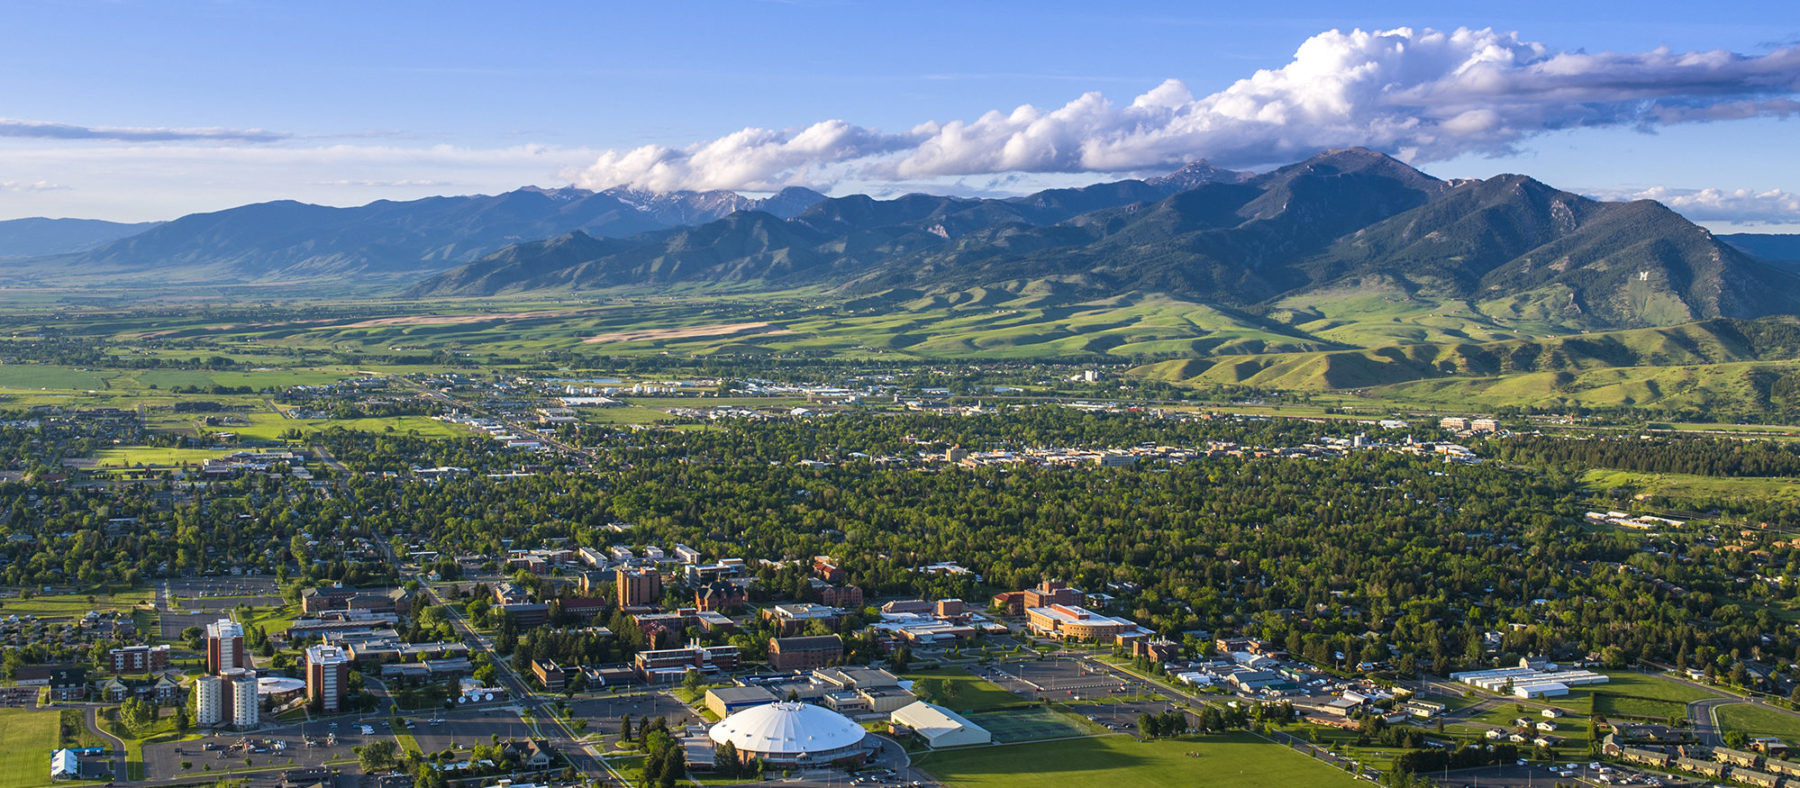
\includegraphics[width=5in,height=\textheight]{images/msu-campus.jpg}}
\usepackage{etoolbox}
\makeatletter
\providecommand{\subtitle}[1]{% add subtitle to \maketitle
  \apptocmd{\@title}{\par {\large #1 \par}}{}{}
}
\makeatother
\subtitle{Spring 2025\\
Montana State University}
\author{Melinda Yager\\
Jade Schmidt\\
Stacey Hancock}
\date{}

\begin{document}
\maketitle

\newpage
\thispagestyle{empty}

This resource was developed by Melinda Yager, Jade Schmidt, and Stacey Hancock in 2021 to accompany the online textbook: Hancock, S., Carnegie, N., Meyer, E., Schmidt, J., and Yager, M. (2021). \emph{Montana State Introductory Statistics with R}. Montana State University. \url{https://mtstateintrostats.github.io/IntroStatTextbook/}.

This resource is released under a \href{https://creativecommons.org/licenses/by-nc-sa/4.0/}{Creative Commons BY-NC-SA 4.0} license unless otherwise noted.

\setcounter{tocdepth}{1}
\addtocontents{toc}{\protect\thispagestyle{empty}}
\tableofcontents
\thispagestyle{empty}

\newpage
\setcounter{page}{1}

\chapter*{Preface}\label{preface}
\addcontentsline{toc}{chapter}{Preface}

This coursepack accompanies the textbook for STAT 216: Montana State Introductory Statistics with R, which can be found at \url{https://mtstateintrostats.github.io/IntroStatTextbook/}. The syllabus for the course (including the course calendar), data sets, and links to D2L Brightspace, Gradescope, and the MSU RStudio server can be found on the course webpage: \url{https://math.montana.edu/courses/s216/}.
Other notes and review materials are linked in D2L.

Each of the activities in this workbook is designed to target specific learning outcomes of the course, giving you practice with important statistical concepts in a group setting with instructor guidance. In addition to the in-class activities for the course, video notes are provided to aid in taking notes while you complete the required videos. Bring this workbook with you to class each class period, and take notes in the workbook as you would your own notes. A well-written completed workbook will provide an optimal study guide for exams!

All activities and labs in this coursepack will be completed during class time. Parts of each lab will be turned in on Gradescope. To aid in your understanding, read through the introduction for each activity before attending class each day.

STAT 216 is a 3-credit in-person course. In our experience, it takes six to nine hours per week outside of class to achieve a good grade in this class. By ``good'' we mean at least a C because a grade of D or below does not count toward fulfilling degree requirements. Many of you set your goals higher than just getting a C, and we fully support that. You need roughly nine hours per week to review past activities, read feedback on previous assignments, complete current assignments, and prepare for the next day's class. A typical week in the life of a STAT 216 student looks like:

\begin{itemize}
\tightlist
\item
  \emph{Prior to class meeting}:

  \begin{itemize}
  \tightlist
  \item
    Read assigned sections of the textbook, using the provided reading guides to take notes on the material.
  \item
    Watch the provided videos, taking notes in the coursepack.
  \item
    Read through the introduction to the day's in-class activity.
  \item
    Read through the week's homework assignment and note any questions you may have on the content.
  \end{itemize}
\item
  \emph{During class meeting}:

  \begin{itemize}
  \tightlist
  \item
    Work through the guided activity, in-class activity or weekly lab with your classmates and instructor, taking detailed notes on your answers to each question in the activity.
  \end{itemize}
\item
  \emph{After class meeting}:

  \begin{itemize}
  \tightlist
  \item
    Complete any parts of the activity you did not complete in class.
  \item
    Review the activity solutions in the Math and Stat Center, and take notes on key points.
  \item
    Complete any remaining assigned readings for the week.
  \item
    Complete the week's homework assignment.
  \end{itemize}
\end{itemize}

\nocite{*}

\chapter{Inference for a Two Categorical Variable: Theory-based Methods}\label{inference-for-a-two-categorical-variable-theory-based-methods}

\section{Vocabulary Review and Key Topics}\label{vocabulary-review-and-key-topics}

Review the Golden Ticket posted in the resources at the end of the coursepack for a summary of a two categorical variables.

\subsection{Key topics}\label{key-topics}

Module 9 introduces theory-based hypothesis testing methods and both simulation-based and theory-based confidence intervals for two categorical variables.

Conditions for the sampling distribution of \(\hat{p}_1-\hat{p}_2\) to follow an approximate normal distribution:

\begin{itemize}
\item
  \textbf{Independence}: The data are independent within and between the two groups. (\emph{Remember}: This also must be true to use simulation methods!)
\item
  \textbf{Success-failure condition}: This condition is met if we have at least 10 successes and 10 failures in each sample. Equivalently, we check that all cells in the table have at least 10 observations.
\item
  Calculation of standard error assuming the null is true:
\end{itemize}

\[SE(\hat{p}_1 - \hat{p}_2) = \sqrt{\hat{p}_{pooled} \times (1-\hat{p}_{pooled}) \times (\frac{1}{n_1}+\frac{1}{n_2})}\]

\begin{itemize}
\tightlist
\item
  Calculation of the standardized difference in sample proportion:
\end{itemize}

\[t = \frac{\hat{p}_1-\hat{p}_2-0}{SE(\hat{p}_1 - \hat{p}_2)}\]

\begin{itemize}
\item
  Measures the number of standard errors the sample difference in proportions is above or below the null value of zero
\item
  Calculation of the difference in sample proportion not assuming the null is true
\end{itemize}

\[SE(\hat{p}_1-\hat{p}_2) = \sqrt{\frac{\hat{p}_1 \times  (1-\hat{p}_1)}{n_1}+\frac{\hat{p}_2 \times  (1-\hat{p}_2)}{n_2}}\]
* Calculation of the confidence interval for a difference in sample proportions

\[\hat{p}_1-\hat{p}_2\pm z^*\times SE(\hat{p}_1-\hat{p}_2)\]
\newpage

\section{Video Notes: Theoretical Inference for Two Categorical Variables}\label{video-notes-theoretical-inference-for-two-categorical-variables}

Read Sections 15.3 and 15.4 in the course textbook. Use the following videos to complete the video notes for Module 9.

\subsection{Course Videos}\label{course-videos}

\begin{itemize}
\item
  15.3TheoryTests
\item
  15.3TheoryIntervals
\end{itemize}

\setstretch{1}

\subsection*{Hypothesis testing using theory-based methods - Video 15.4TheoryTests}\label{hypothesis-testing-using-theory-based-methods---video-15.4theorytests}
\addcontentsline{toc}{subsection}{Hypothesis testing using theory-based methods - Video 15.4TheoryTests}

Example: In Modules 3 and 4, we investigated data on higher education institutions in the United States, collected by the Integrated Postsecondary Education Data System (IPEDS) for the National Center for Education Statistics (NCES) (Education Statistics 2018). A random sample of 2900+ higher education institutions in the United States was collected in 2018. Two variables measured on this data set is whether the institution is a land grant university and whether the institution offers tenure. Does the proportion of universities that offer tenure differ between land grant and non-land-grant institutions?

What is the explanatory variable?

\vspace{0.2in}

What is the response variable?

\vspace{0.2in}

Write the parameter of interest:

\vspace{0.8in}

Hypotheses:

In notation:

\(H_0:\)

\vspace{0.2in}

\(H_A:\)

\vspace{0.2in}

\begin{Shaded}
\begin{Highlighting}[]
\NormalTok{IPED }\OtherTok{\textless{}{-}}\FunctionTok{read.csv}\NormalTok{(}\StringTok{"https://math.montana.edu/courses/s216/data/IPEDS\_2018.csv"}\NormalTok{)}

\NormalTok{IPEDS }\OtherTok{\textless{}{-}}\NormalTok{ IPED }\SpecialCharTok{\%\textgreater{}\%}
    \FunctionTok{drop\_na}\NormalTok{(Tenure)}

\NormalTok{IPEDS }\SpecialCharTok{\%\textgreater{}\%} \CommentTok{\# Data set piped into...}
    \FunctionTok{ggplot}\NormalTok{(}\FunctionTok{aes}\NormalTok{(}\AttributeTok{x =}\NormalTok{ LandGrant, }\AttributeTok{fill =}\NormalTok{ Tenure)) }\SpecialCharTok{+}   \CommentTok{\# This specifies the variables}
  \FunctionTok{geom\_bar}\NormalTok{(}\AttributeTok{stat =} \StringTok{"count"}\NormalTok{, }\AttributeTok{position =} \StringTok{"fill"}\NormalTok{) }\SpecialCharTok{+}  \CommentTok{\# Tell it to make a stacked bar plot}
  \FunctionTok{labs}\NormalTok{(}\AttributeTok{title =} \StringTok{"Segmented Bar Plot of Tenure Availability }
\StringTok{       by Type of Institution for Higher Ed Institutions"}\NormalTok{,  }
       \CommentTok{\# Make sure to title your plot }
       \AttributeTok{x =} \StringTok{"Land Grant"}\NormalTok{,   }\CommentTok{\# Label the x axis}
       \AttributeTok{y =} \StringTok{""}\NormalTok{) }\SpecialCharTok{+} \CommentTok{\# Remove y axis label }
    \FunctionTok{scale\_fill\_grey}\NormalTok{()}

\NormalTok{IPEDS }\SpecialCharTok{\%\textgreater{}\%} \FunctionTok{group\_by}\NormalTok{(LandGrant) }\SpecialCharTok{\%\textgreater{}\%} \FunctionTok{count}\NormalTok{(Tenure)}
\end{Highlighting}
\end{Shaded}

\begin{verbatim}
#> # A tibble: 4 x 3
#> # Groups:   LandGrant [2]
#>   LandGrant Tenure     n
#>   <chr>     <chr>  <int>
#> 1 No        No       976
#> 2 No        Yes     1829
#> 3 Yes       No        31
#> 4 Yes       Yes       72
\end{verbatim}

\begin{center}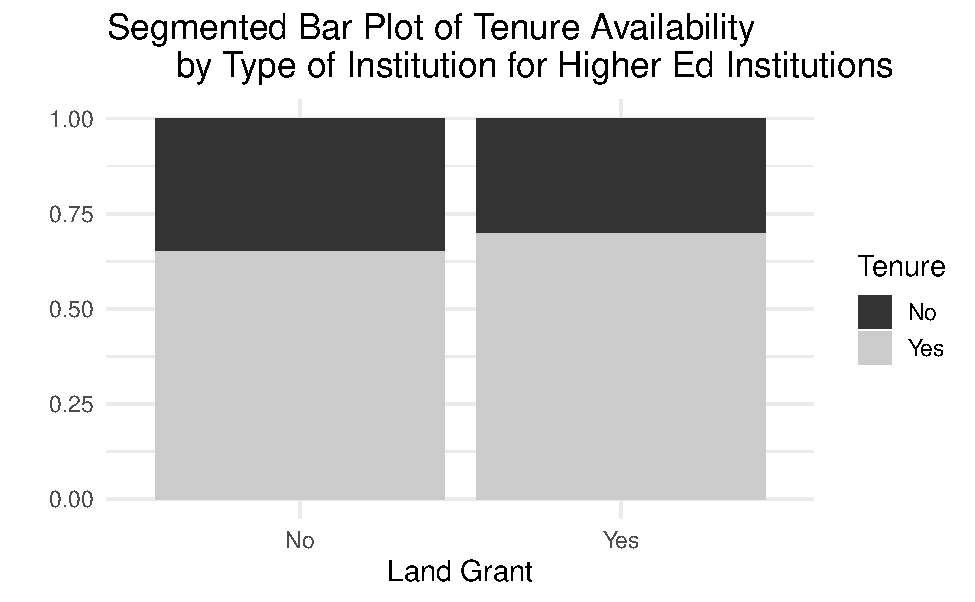
\includegraphics[width=0.7\linewidth]{09-VN09-two-cat-theory_files/figure-latex/unnamed-chunk-1-1} \end{center}

Report the summary statistic:

\vspace{0.6in}

Conditions for inference using theory-based methods for two categorical variables:

\begin{itemize}
\tightlist
\item
  Independence: the response for one observational unit will not influence another observational unit
\end{itemize}

\vspace{0.2in}

\begin{itemize}
\tightlist
\item
  Large enough sample size:
\end{itemize}

\vspace{0.7in}

Are the conditions met to analyze the university data using theory-based methods?

\vspace{0.8in}
\newpage

Steps to use theory-based methods:

\begin{itemize}
\item
  Calculate the standardized statistic
\item
  Find the area under the standard normal distribution at least as extreme as the standardized statistic
\end{itemize}

Equation for the standard error of the difference in sample proportions assuming the null hypothesis is true:

\vspace{0.8in}

\setstretch{1.5}

\begin{itemize}
\tightlist
\item
  This value measures how far each possible sample difference in proportions is from the null value, on average.
\end{itemize}

\setstretch{1}

Equation for the standardized difference in sample proportions:

\vspace{0.8in}

\setstretch{1.5}

\begin{itemize}
\tightlist
\item
  This value measures how many standard errors the sample difference in proportions is above/below the null value.
\end{itemize}

\setstretch{1}

Calculate the standardized difference in sample proportion of higher education institutions that offer tenure between land grant universities and non-land grant universities.

\begin{itemize}
\tightlist
\item
  First calculate the standard error of the difference in proportion assuming the null hypothesis is true
\end{itemize}

\vspace{0.4in}

\begin{itemize}
\tightlist
\item
  Then calculate the Z score
\end{itemize}

\vspace{0.4in}

\begin{center}\includegraphics[width=0.5\linewidth]{09-VN09-two-cat-theory_files/figure-latex/standNormc-1} \end{center}

Interpret the standardized statistic

\vspace{0.5in}

\newpage

To find the p-value, find the area under the standard normal distribution at the standardized statistic and more extreme.

\begin{Shaded}
\begin{Highlighting}[]
\FunctionTok{pnorm}\NormalTok{(}\FloatTok{0.985}\NormalTok{, }\AttributeTok{lower.tail =} \ConstantTok{FALSE}\NormalTok{)}\SpecialCharTok{*}\DecValTok{2}
\end{Highlighting}
\end{Shaded}

\begin{verbatim}
#> [1] 0.3246241
\end{verbatim}

Interpretation of the p-value:

\begin{itemize}
\item
  Statement about probability or proportion of samples
\item
  Statistic (summary measure and value)
\item
  Direction of the alternative
\item
  Null hypothesis (in context)
\end{itemize}

\vspace{0.8in}

Conclusion with scope of inference:

\begin{itemize}
\item
  Amount of evidence
\item
  Parameter of interest
\item
  Direction of the alternative hypothesis
\item
  Generalization
\item
  Causation
\end{itemize}

\vspace{0.6in}

\subsection*{Confidence interval - Video 15.3TheoryIntervals}\label{confidence-interval---video-15.3theoryintervals}
\addcontentsline{toc}{subsection}{Confidence interval - Video 15.3TheoryIntervals}

\begin{itemize}
\item
  Estimate the \_\_\_\_\_\_\_\_\_\_\_\_\_\_\_ in true \_\_\_\_\_\_\_\_\_\_\_\_\_\_\_
\item
  \(CI = \text{statistic} \pm \text{margin of error}\)
\end{itemize}

\subsubsection*{Theory-based method for a two categorical variables}\label{theory-based-method-for-a-two-categorical-variables}
\addcontentsline{toc}{subsubsection}{Theory-based method for a two categorical variables}

\begin{itemize}
\tightlist
\item
  \(CI = \hat{p}_1-\hat{p}_2 \pm (z^* \times SE(\hat{p}_1-\hat{p}_2))\)
\end{itemize}

\setstretch{1.5}

\begin{itemize}
\tightlist
\item
  When creating a confidence interval, we no longer assume the \_\_\_\_\_\_\_\_\_\_\_\_\_ hypothesis is true. Use the sample \_\_\_\_\_\_\_\_\_\_\_\_\_ to calculate the sample to sample variability, rather than \(\hat{p}_{pooled}\).
\end{itemize}

\setstretch{1}

Equation for the standard error of the difference in sample proportions \emph{NOT} assuming the null is true:

\vspace{0.6in}

\newpage

Example: Estimate the difference in true proportions of higher education institutions that offer tenure between land grant universities and non-land grant universities.

Find a 90\% confidence interval:

\begin{itemize}
\tightlist
\item
  1st find the \(z^*\) multiplier
\end{itemize}

\begin{Shaded}
\begin{Highlighting}[]
\FunctionTok{qnorm}\NormalTok{(}\FloatTok{0.95}\NormalTok{, }\AttributeTok{lower.tail=}\ConstantTok{TRUE}\NormalTok{)}
\end{Highlighting}
\end{Shaded}

\begin{verbatim}
#> [1] 1.644854
\end{verbatim}

\begin{itemize}
\tightlist
\item
  Next, calculate the standard error for the difference in proportions \textbf{NOT} assuming the null hypothesis is true
\end{itemize}

\vspace{0.8in}

\begin{itemize}
\tightlist
\item
  Calculate the margin of error
\end{itemize}

\vspace{0.6in}

\begin{itemize}
\tightlist
\item
  Calculate the endpoints of the 90\% confidence interval
\end{itemize}

\vspace{0.6in}

Confidence interval interpretation:

\begin{itemize}
\item
  How confident you are (e.g., 90\%, 95\%, 98\%, 99\%)
\item
  Parameter of interest
\item
  Calculated interval
\item
  Order of subtraction when comparing two groups
\end{itemize}

\vspace{0.8in}

\subsection{Concept Check}\label{concept-check}

Be prepared for group discussion in the next class. One member from the table should write the answers to the following on the whiteboard.

\begin{enumerate}
\def\labelenumi{\arabic{enumi}.}
\tightlist
\item
  What conditions must be met to use the Normal Distribution to approximate the sampling distribution for the difference in sample proportions?
\end{enumerate}

\vspace{0.8in}

\begin{enumerate}
\def\labelenumi{\arabic{enumi}.}
\setcounter{enumi}{1}
\tightlist
\item
  Explain why a theory-based confidence interval for the Good Samaritan study from last module would NOT be similar to the bootstrap interval created.
\end{enumerate}

\vspace{1in}

\newpage

\section{Activity 19: Winter Sports Helmet Use and Head Injuries --- Theory-based Methods}\label{activity-19-winter-sports-helmet-use-and-head-injuries-theory-based-methods}

\setstretch{1}

\subsection{Learning outcomes}\label{learning-outcomes}

\begin{itemize}
\item
  Assess the conditions to use the normal distribution model for a difference in proportions.
\item
  Create and interpret a theory-based confidence interval for a difference in proportions.
\item
  Calculate and interpret the standardized difference in sample proportion
\item
  Use the standard normal distribution to find the p-value for the test
\end{itemize}

\subsection{Terminology review}\label{terminology-review}

In today's activity, we will use theory-based methods to estimate the difference in two proportions. Some terms covered in this activity are:

\begin{itemize}
\item
  Standard normal distribution
\item
  Independence and success-failure conditions
\end{itemize}

To review these concepts, see Chapter 15 in your textbook.

\subsection{Winter sports helmet use and head injury}\label{winter-sports-helmet-use-and-head-injury}

In this activity we will focus on theory-based methods to calculate a confidence interval. The sampling distribution of a difference in proportions can be mathematically modeled using the normal distribution if certain conditions are met.

Conditions for the sampling distribution of \(\hat{p}_1-\hat{p}_2\) to follow an approximate normal distribution:

\begin{itemize}
\item
  \textbf{Independence}: The data are independent within and between the two groups. (\emph{Remember}: This also must be true to use simulation methods!)
\item
  \textbf{Success-failure condition}: This condition is met if we have at least 10 successes and 10 failures in each sample. Equivalently, we check that all cells in the table have at least 10 observations.
\end{itemize}

A study was reported in ``Helmet Use and Risk of Head Injuries in Alpine Skiers and Snowboarders'' by Sullheim et. al., (Sulheim et al. 2017), on the use of helmets and head injuries for skiers and snowboarders involved in accidents. The summary results from a random sample of 3562 skiers and snowboarders involved in accidents is shown in the two-way table below.

\begin{longtable}[]{@{}cccc@{}}
\toprule\noalign{}
& Helmet Use & No Helmet Use & Total \\
\midrule\noalign{}
\endhead
\bottomrule\noalign{}
\endlastfoot
Head Injury & 96 & 480 & 576 \\
No Head Injury & 656 & 2330 & 2986 \\
Total & 752 & 2810 & 3562 \\
\end{longtable}

\begin{itemize}
\item
  Download the R script file from D2L and upload to the RStudio server
\item
  Highlight and run 1--13 to import the data set and create the segmented bar plot
\end{itemize}

\begin{Shaded}
\begin{Highlighting}[]
\NormalTok{skiers }\OtherTok{\textless{}{-}} \FunctionTok{read.csv}\NormalTok{(}\StringTok{"https://www.math.montana.edu/courses/s216/data/HeadInjuries.csv"}\NormalTok{) }\CommentTok{\# Read data set in}
\NormalTok{skiers }\SpecialCharTok{\%\textgreater{}\%} \CommentTok{\# Data set piped into...}
  \FunctionTok{ggplot}\NormalTok{(}\FunctionTok{aes}\NormalTok{(}\AttributeTok{x =}\NormalTok{ Helmet, }\AttributeTok{fill =}\NormalTok{ Outcome)) }\SpecialCharTok{+}   \CommentTok{\# This specifies the variables}
  \FunctionTok{geom\_bar}\NormalTok{(}\AttributeTok{stat =} \StringTok{"count"}\NormalTok{, }\AttributeTok{position =} \StringTok{"fill"}\NormalTok{) }\SpecialCharTok{+}  \CommentTok{\# Tell it to make a stacked bar plot}
  \FunctionTok{labs}\NormalTok{(}\AttributeTok{title =} \StringTok{"Segmented Bar Plot of Head Injuries for Skiers/Snowboarders}
\StringTok{       Involved in Injuries between Helmet Use"}\NormalTok{,  }\CommentTok{\# Make sure to title your plot}
       \AttributeTok{x =} \StringTok{"Helmet Use"}\NormalTok{,   }\CommentTok{\# Label the x axis}
       \AttributeTok{y =} \StringTok{""}\NormalTok{) }\SpecialCharTok{+}  \CommentTok{\# Remove y axis label}
  \FunctionTok{scale\_fill\_grey}\NormalTok{()  }\CommentTok{\# Make figure black and white}
\end{Highlighting}
\end{Shaded}

\begin{center}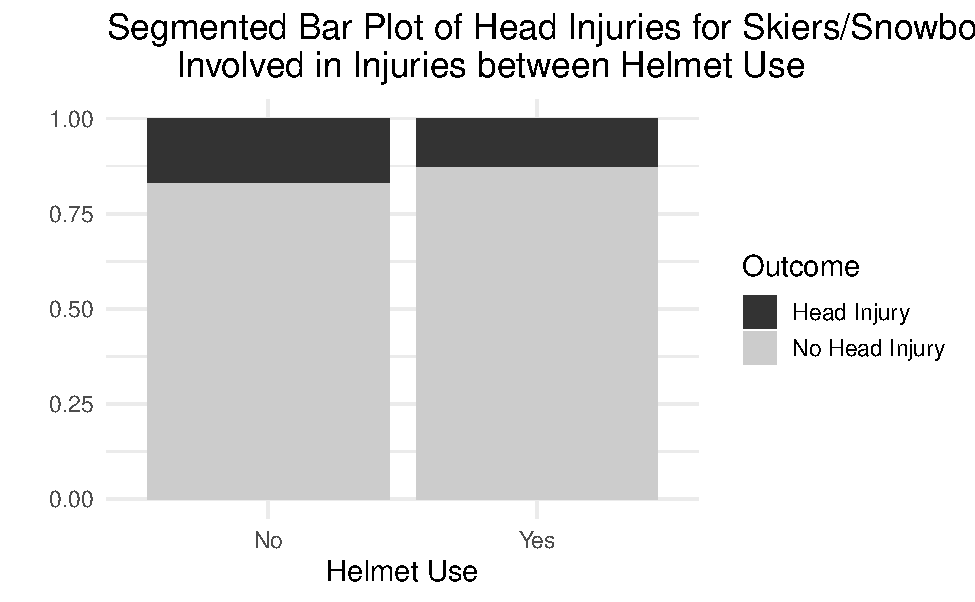
\includegraphics[width=0.6\linewidth]{09-A19-inference-2cat-theory_files/figure-latex/unnamed-chunk-1-1} \end{center}

\begin{enumerate}
\def\labelenumi{\arabic{enumi}.}
\tightlist
\item
  Verify the independence condition is met.
\end{enumerate}

\vspace{0.6in}

\begin{enumerate}
\def\labelenumi{\arabic{enumi}.}
\setcounter{enumi}{1}
\tightlist
\item
  Verify the success failure condition is met to use theory-based methods.
\end{enumerate}

\vspace{1in}

\begin{enumerate}
\def\labelenumi{\arabic{enumi}.}
\setcounter{enumi}{2}
\tightlist
\item
  Calculate the difference in sample proportion of skiers and snowboarders involved in accidents with a head injury for those who wear helmets and those who do not. Use appropriate notation with informative subscripts.
\end{enumerate}

\vspace{0.8in}

\subsubsection*{Hypothesis test}\label{hypothesis-test}
\addcontentsline{toc}{subsubsection}{Hypothesis test}

\begin{enumerate}
\def\labelenumi{\arabic{enumi}.}
\setcounter{enumi}{3}
\tightlist
\item
  Write the null and alternative hypotheses in notation.
\end{enumerate}

~~~\(H_0\):

\vspace{0.2in}

~~~\(H_A\):

\vspace{0.2in}

\subsubsection*{Use statistical analysis methods to draw inferences from the data}\label{use-statistical-analysis-methods-to-draw-inferences-from-the-data}
\addcontentsline{toc}{subsubsection}{Use statistical analysis methods to draw inferences from the data}

To test the null hypothesis, we could use simulation-based methods as we did in the activities in Module 8. In this activity, we will focus on theory-based methods. Like with a single proportion, the sampling distribution of a difference in sample proportions can be mathematically modeled using the normal distribution if certain conditions are met.

To calculate the standardized statistic we use:

\[
Z = \frac{(\hat{p_1} - \hat{p_2}) - \text{null value}}{SE_0(\hat{p_1}-\hat{p}_2)},
\]

where the null standard error is calculated using the pooled proportion of successes:

\[
SE_0(\hat{p}_1-\hat{p}_2)=\sqrt{\hat{p}_{pool}\times (1-\hat{p}_{pool})\times \left(\frac{1}{n_1}+\frac{1}{n_2}\right)}.
\]
For this study we would first calculate the pooled proportion of successes.

\[\hat{p}_{pool} = \frac{\text{number of "successes"}}{\text{number of cases}} \]
\vspace{1mm}

\begin{enumerate}
\def\labelenumi{\arabic{enumi}.}
\setcounter{enumi}{4}
\tightlist
\item
  Calculate the pooled proportion of head injuries.
\end{enumerate}

\vspace{1in}

\begin{enumerate}
\def\labelenumi{\arabic{enumi}.}
\setcounter{enumi}{5}
\tightlist
\item
  Use the value for the pooled proportion of successes to calculate the \(SE_0(\hat{p}_1 - \hat{p}_2)\) assuming the null hypothesis is true.
\end{enumerate}

\vspace{1in}

\begin{enumerate}
\def\labelenumi{\arabic{enumi}.}
\setcounter{enumi}{6}
\tightlist
\item
  Use the value of the null standard error to calculate the standardized statistic (standardized difference in proportion).
\end{enumerate}

\vspace{1in}

\newpage

\begin{enumerate}
\def\labelenumi{\arabic{enumi}.}
\setcounter{enumi}{7}
\tightlist
\item
  Mark the value of the standardized difference in proportion on the standard normal distribution shown below. Interpret the standardized statistic in context of the problem.
\end{enumerate}

\vspace{1mm}

\begin{center}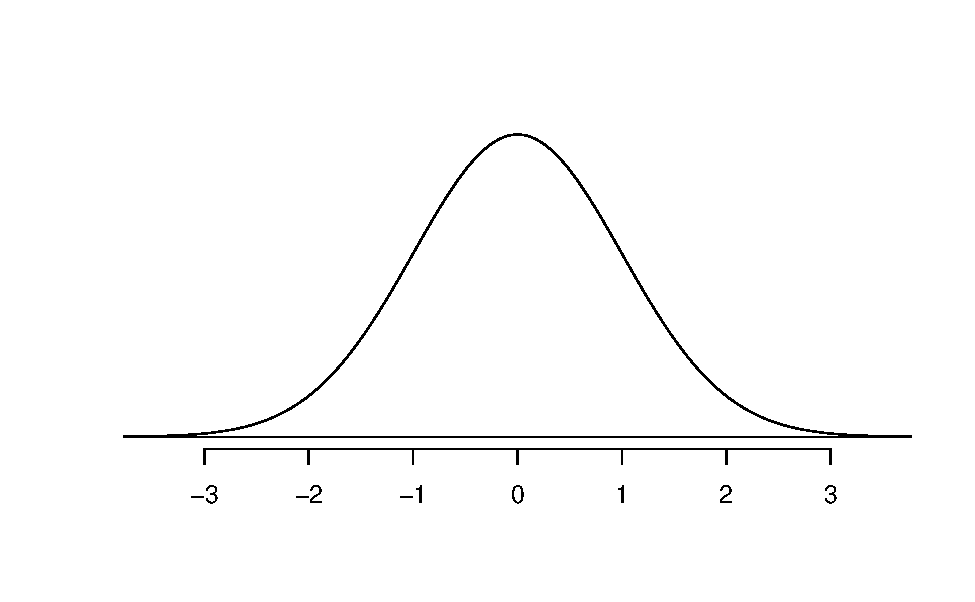
\includegraphics[width=0.5\linewidth]{09-A19-inference-2cat-theory_files/figure-latex/simpleNormal-1} \end{center}

\vspace{0.6in}

We will use the \texttt{pnorm()} function in R to find the p-value.

\begin{itemize}
\item
  Enter the value of z from question 7 for xx
\item
  Highlight and run lines 18--20
\end{itemize}

\begin{Shaded}
\begin{Highlighting}[]
\FunctionTok{pnorm}\NormalTok{(xx, }\CommentTok{\# Enter value of standardized statistic}
      \AttributeTok{m=}\DecValTok{0}\NormalTok{, }\AttributeTok{s=}\DecValTok{1}\NormalTok{, }\CommentTok{\# Using the standard normal mean = 0, sd = 1}
      \AttributeTok{lower.tail=}\ConstantTok{TRUE}\NormalTok{) }\CommentTok{\# Gives a p{-}value less than the standardized statistic}
\end{Highlighting}
\end{Shaded}

\begin{enumerate}
\def\labelenumi{\arabic{enumi}.}
\setcounter{enumi}{8}
\tightlist
\item
  Write a conclusion to the test.
\end{enumerate}

\vspace{1in}

\subsection*{How would an increase in sample size impact the p-value of the test?}\label{how-would-an-increase-in-sample-size-impact-the-p-value-of-the-test}
\addcontentsline{toc}{subsection}{How would an increase in sample size impact the p-value of the test?}

\begin{longtable}[]{@{}cccc@{}}
\toprule\noalign{}
& Helmet Use & No Helmet Use & Total \\
\midrule\noalign{}
\endhead
\bottomrule\noalign{}
\endlastfoot
Head Injury & 135 & 674 & 809 \\
No Head Injury & 921 & 3270 & 4191 \\
Total & 1056 & 3944 & 5000 \\
\end{longtable}

Note that the sample proportions for each group are the same as the smaller sample size.

\[\hat{p}_h = \frac{135}{1056}=0.128, \hspace{2mm} \hat{p}_n = \frac{674}{3944}=0.171\]

First calculate the pooled proportion of successes.

\[\hat{p}_{pool} = \frac{\text{number of "successes"}}{\text{number of cases}} = \frac{809}{5000} = 0.162\]

We use the value for the pooled proportion of successes to calculate the \(SE_0(\hat{p}_1 - \hat{p}_2)\).

\[
SE_0(\hat{p}_1-\hat{p}_2)=\sqrt{0.162 \times (1-0.162)\times \left(\frac{1}{1056}+\frac{1}{3944}\right)} = 0.013
\]
Standardized Statistic Calculation:

\[Z = \frac{0.128 - 0.171 - 0}{0.013} = -3.308\]

Use Rstudio to find the p-value for this new sample.

\begin{Shaded}
\begin{Highlighting}[]
\FunctionTok{pnorm}\NormalTok{(}\SpecialCharTok{{-}}\FloatTok{3.308}\NormalTok{, }\CommentTok{\# Enter value of standardized statistic}
      \AttributeTok{m=}\DecValTok{0}\NormalTok{, }\AttributeTok{s=}\DecValTok{1}\NormalTok{, }\CommentTok{\# Using the standard normal mean = 0, sd = 1}
      \AttributeTok{lower.tail=}\ConstantTok{TRUE}\NormalTok{) }\CommentTok{\# Gives a p{-}value greater than the standardized statistic}
\end{Highlighting}
\end{Shaded}

\begin{verbatim}
#> [1] 0.000469824
\end{verbatim}

\begin{enumerate}
\def\labelenumi{\arabic{enumi}.}
\setcounter{enumi}{9}
\tightlist
\item
  How does the increase in sample size affect the p-value?
\end{enumerate}

\vspace{0.4in}

\vspace{.8in}

\subsection{Take-home messages}\label{take-home-messages}

\begin{enumerate}
\def\labelenumi{\arabic{enumi}.}
\item
  Simulation-based methods and theory-based methods should give similar results for a study \emph{if the validity conditions are met}. For both methods, observational units need to be independent. To use theory-based methods, additionally, the success-failure condition must be met. Check the validity conditions for each type of test to determine if theory-based methods can be used.
\item
  When calculating the standard error for the difference in sample proportions when doing a hypothesis test, we use the pooled proportion of successes, the best estimate for calculating the variability \emph{under the assumption the null hypothesis is true}.
\item
  Increasing sample size will result in less sample-to-sample variability in statistics, which will result in a smaller standard error, and a larger standardized statistic.
\end{enumerate}

\subsection{Additional notes}\label{additional-notes}

Use this space to summarize your thoughts and take additional notes on today's activity and material covered.

\newpage

\section{Activity 20: Diabetes}\label{activity-20-diabetes}

\setstretch{1}

\subsection{Learning outcomes}\label{learning-outcomes-1}

\begin{itemize}
\item
  Assess the conditions to use the normal distribution model for a difference in proportions.
\item
  Describe and perform a simulation-based confidence interval for a difference in proportions.
\item
  Create and interpret a theory-based confidence interval for a difference in proportions.
\end{itemize}

\subsection{Glycemic control in diabetic adolescents}\label{glycemic-control-in-diabetic-adolescents}

Researchers compared the efficacy of two treatment regimens to achieve durable glycemic control in children and adolescents with recent-onset type 2 diabetes (Group 2012). A convenience sample of patients 10 to 17 years of age with recent-onset type 2 diabetes were randomly assigned to either a medication (rosiglitazone) or a lifestyle-intervention program focusing on weight loss through eating and activity. Researchers measured whether the patient still needs insulin (failure) or had glycemic control (success). Of the 233 children who received the Rosiglitazone treatment, 143 had glycemic control, while of the 234 who went through the lifestyle-intervention program, 125 had glycemic control. Is there evidence that there is difference in proportion of patients that achieve durable glycemic control between the two treatments? Use Rosiglitazone -- Lifestyle as the order of subtraction.

\begin{itemize}
\item
  Upload and open the R script file. Upload the csv file, \texttt{diabetes}.
\item
  Enter the name of the data set for \texttt{datasetname.csv} in the R script file in line 7.
\item
  Highlight and run lines 1--8 to get the counts for each combination of categories.
\end{itemize}

\begin{Shaded}
\begin{Highlighting}[]
\NormalTok{glycemic }\OtherTok{\textless{}{-}} \FunctionTok{read.csv}\NormalTok{(}\StringTok{"datasetname.csv"}\NormalTok{)}
\NormalTok{glycemic }\SpecialCharTok{\%\textgreater{}\%} \FunctionTok{group\_by}\NormalTok{(treatment) }\SpecialCharTok{\%\textgreater{}\%} \FunctionTok{count}\NormalTok{(outcome)}
\end{Highlighting}
\end{Shaded}

\begin{enumerate}
\def\labelenumi{\arabic{enumi}.}
\item
  Is this an experiment or an observational study?
  \vspace{0.2in}
\item
  Complete the following two-way table using the R output.
\end{enumerate}

\begin{center}
\begin{tabular}{|c|c|c|c|}\hline
 & \multicolumn{2}{|c|}{\textbf{Treatment}} & \\ \hline
\textbf{Outcome} & \hspace{0.35in} rosiglitazone \hspace{0.35in} & \hspace{0.35in} lifestyle \hspace{0.35in} & \hspace{0.35in} Total \hspace{0.35in} \\ \hline
 glycemic control & & & \\ 
 (success) & & & \\ \hline
 insulin required & & & \\ 
 (failure) & & & \\ \hline
 Total & & &  \\ 
 & & & \\ \hline  
\end{tabular}
\end{center}

\begin{enumerate}
\def\labelenumi{\arabic{enumi}.}
\setcounter{enumi}{2}
\item
  Is the independence condition met for this study? Explain your answer.
  \vspace{0.6in}
\item
  Is the success failure condition met for this study? Explain your answer.
\end{enumerate}

\vspace{0.6in}

\begin{enumerate}
\def\labelenumi{\arabic{enumi}.}
\setcounter{enumi}{4}
\item
  Write the parameter of interest for the research question.
  \vspace{0.6in}
\item
  \textbf{Calculate the summary statistic (difference in proportions). Use appropriate notation.}
  \vspace{0.3in}
\end{enumerate}

\subsection*{Simulation methods}\label{simulation-methods}
\addcontentsline{toc}{subsection}{Simulation methods}

First we will use simulation methods to find the confidence interval. This will give an interval estimate for the parameter of inference.

We will use the \texttt{two\_proportion\_bootstrap\_CI()} function in R (in the \texttt{catstats} package) to simulate the bootstrap distribution of differences in sample proportions and calculate a 90\% confidence interval. We will need to enter the response variable name and the explanatory variable name for the formula, the data set name (identified above as \texttt{glycemic}), the outcome for the explanatory variable that is first in subtraction, number of repetitions, the outcome for the response variable that is a success (what the numerator counts when calculating a sample proportion), and the confidence level as a decimal.

\begin{enumerate}
\def\labelenumi{\arabic{enumi}.}
\setcounter{enumi}{6}
\tightlist
\item
  What inputs should be entered for each of the following to create the bootstrap simulation?
  \vspace{1mm}
\end{enumerate}

\begin{itemize}
\tightlist
\item
  First in subtraction (What is the outcome for the explanatory variable that is used as first in the order of subtraction? \texttt{"rosi"} or \texttt{"lifestyle"}):
\end{itemize}

\vspace{.15in}

\begin{itemize}
\tightlist
\item
  Number of repetitions:
\end{itemize}

\vspace{.15in}

\begin{itemize}
\tightlist
\item
  Response value numerator (What is the outcome for the response variable that is considered a success? \texttt{"success"} or \texttt{"failure"}):
\end{itemize}

\vspace{.15in}

\begin{itemize}
\tightlist
\item
  confidence\_level:
\end{itemize}

\vspace{.15in}

\begin{itemize}
\item
  Fill in the missing values/names in the R script file in the two\_proportion\_bootstrap\_CI function to create a simulation 90\% confidence interval.
\item
  Highlight and run lines 12--17
\end{itemize}

\begin{Shaded}
\begin{Highlighting}[]
\FunctionTok{two\_proportion\_bootstrap\_CI}\NormalTok{(}\AttributeTok{formula =}\NormalTok{ response}\SpecialCharTok{\textasciitilde{}}\NormalTok{explanatory, }
         \AttributeTok{data=}\NormalTok{glycemic, }\CommentTok{\# Name of data set}
         \AttributeTok{first\_in\_subtraction =} \StringTok{"xx"}\NormalTok{, }\CommentTok{\# Order of subtraction: enter the name of Group 1}
         \AttributeTok{response\_value\_numerator =} \StringTok{"xx"}\NormalTok{, }\CommentTok{\# Define which outcome is a success }
         \AttributeTok{number\_repetitions =} \DecValTok{1000}\NormalTok{, }\CommentTok{\# Always use a minimum of 1000 repetitions}
         \AttributeTok{confidence\_level =}\NormalTok{ xx) }\CommentTok{\# Enter the level of confidence as a decimal}
\end{Highlighting}
\end{Shaded}

\begin{enumerate}
\def\labelenumi{\arabic{enumi}.}
\setcounter{enumi}{7}
\tightlist
\item
  Report the 90\% confidence interval.
\end{enumerate}

\vspace{0.3in}

\begin{enumerate}
\def\labelenumi{\arabic{enumi}.}
\setcounter{enumi}{8}
\tightlist
\item
  Interpret the confidence interval in context of the problem.
\end{enumerate}

\vspace{1in}

\newpage

\subsection*{Theory-based Methods}\label{theory-based-methods}
\addcontentsline{toc}{subsection}{Theory-based Methods}

Next we will use theory-based methods to find the 90\% confidence interval. Review the conditions for using theory-based methods from Activity 19.

\begin{enumerate}
\def\labelenumi{\arabic{enumi}.}
\setcounter{enumi}{9}
\tightlist
\item
  Is the sample size large enough to use theory-based methods to find the confidence interval? Explain in context of the study,
\end{enumerate}

\vspace{1.0in}

To find a confidence interval for the difference in proportions we will add and subtract the margin of error from the point estimate to find the two endpoints.

\[\hat{p}_1-\hat{p}_2\pm z^*\times SE(\hat{p}_1-\hat{p}_2), \hspace{.2cm} \text{where}\]
\[SE(\hat{p}_1-\hat{p}_2) = \sqrt{\frac{\hat{p}_1 \times  (1-\hat{p}_1)}{n_1}+\frac{\hat{p}_2 \times  (1-\hat{p}_2)}{n_2}}\]

In this formula, we use the sample proportions for each group to calculate the standard error for the difference in proportions since we are not assuming that the true difference is zero.

\begin{enumerate}
\def\labelenumi{\arabic{enumi}.}
\setcounter{enumi}{10}
\tightlist
\item
  Calculate the standard error of the sample proportion not assuming the null hypothesis is true.
\end{enumerate}

\vspace{0.5in}

Recall that the \(z^*\) multiplier is the percentile of a standard normal distribution that corresponds to our confidence level. If our confidence level is 90\%, we find the Z values that encompass the middle 90\% of the standard normal distribution. If 90\% of the standard normal distribution should be in the middle, that leaves 10\% in the tails, or 5\% in each tail. The \texttt{qnorm()} function in R will tell us the \(z^*\) value for the desired percentile (in this case, 90\% + 5\% = 95\% percentile).

\begin{Shaded}
\begin{Highlighting}[]
\FunctionTok{qnorm}\NormalTok{(}\FloatTok{0.95}\NormalTok{, }\AttributeTok{lower.tail =} \ConstantTok{TRUE}\NormalTok{) }\CommentTok{\# Multiplier for 90\% confidence interval}
\end{Highlighting}
\end{Shaded}

\begin{verbatim}
#> [1] 1.644854
\end{verbatim}

\begin{enumerate}
\def\labelenumi{\arabic{enumi}.}
\setcounter{enumi}{11}
\tightlist
\item
  Mark the value of the \(z^*\) multiplier and the percentages used to find this multiplier on the standard normal distribution shown below.
\end{enumerate}

\begin{center}\includegraphics[width=0.45\linewidth]{09-A20-inference-2cat-CIs_files/figure-latex/standNormc-1} \end{center}

\vspace{1mm}

\newpage

Remember that the margin of error is the value added and subtracted to the sample difference in proportions to find the endpoints for the confidence interval.

\[ME = z^*\times SE(\hat{p}_1 - \hat{p}_2)\]

\begin{enumerate}
\def\labelenumi{\arabic{enumi}.}
\setcounter{enumi}{12}
\tightlist
\item
  Using the multiplier of \(z^*\) = 1.645 and the calculated standard error, calculate the margin of error for a 90\% confidence interval.
\end{enumerate}

\vspace{0.8in}

\begin{enumerate}
\def\labelenumi{\arabic{enumi}.}
\setcounter{enumi}{13}
\tightlist
\item
  Calculate the 90\% confidence interval for the parameter of interest.
\end{enumerate}

\vspace{1in}

\subsection{Take-home messages}\label{take-home-messages-1}

\begin{enumerate}
\def\labelenumi{\arabic{enumi}.}
\item
  When calculating the standard error for the difference in sample proportions when doing a hypothesis test, we use the pooled proportion of successes, the best estimate for calculating the variability \emph{under the assumption the null hypothesis is true}. For a confidence interval, we are not assuming a null hypothesis, so we use the values of the two conditional proportions to calculate the standard error. Make note of the difference in these two formulas.
\item
  Increasing sample size will result in less sample-to-sample variability in statistics, which will result in a smaller standard error, and a larger standardized statistic.
\item
  Since we add and subtract the margin of error to the point estimate, the margin of error is half the width of the confidence interval.
\end{enumerate}

\subsection{Additional notes}\label{additional-notes-1}

Use this space to summarize your thoughts and take additional notes on today's activity and material covered.

\newpage

\section{Module 9 Lab: Poisonous Mushrooms}\label{module-9-lab-poisonous-mushrooms}

\setstretch{1}

\subsection{Learning outcomes}\label{learning-outcomes-2}

\begin{itemize}
\item
  Given a research question involving two categorical variables, construct the null and alternative hypotheses
  in words and using appropriate statistical symbols.
\item
  Describe and perform a simulation-based hypothesis test for a difference in proportions.
\item
  Interpret and evaluate a p-value for a simulation-based hypothesis test for a difference in proportions.
\item
  Interpret and evaluate a confidence interval for a simulation-based confidence interval for a difference in proportions.
\end{itemize}

\subsection{Poisonous Mushrooms}\label{poisonous-mushrooms}

Wild mushrooms, such as chanterelles or morels, are delicious, but eating wild mushrooms carries the risk of accidental poisoning. Even a single bite of the wrong mushroom can be enough to cause fatal poisoning. An amateur mushroom hunter is interested in finding an easy rule to differentiate poisonous and edible mushrooms. They think that the mushroom's gills (the part which holds and releases spores) might be related to a mushroom's edibility. They used a data set of 8124 mushrooms and their descriptions. For each mushroom, the data set includes whether it is edible (e) or poisonous (p) and the size of the gills (broad (b) or narrow (n)). Is there evidence gill size is associated with whether a mushroom is poisonous? PLEASE NOTE: According to The Audubon Society Field Guide to North American Mushrooms, there is no simple rule for determining the edibility of a mushroom; no rule like ``leaflets three, let it be'\,' for Poisonous Oak and Ivy.

\begin{itemize}
\item
  Upload and open the R script file for the Module 9 lab. Upload and import the csv file, \texttt{mushrooms\_edibility}.
\item
  Enter the name of the data set (see the environment tab) for datasetname.csv in the R script file in line 8.
\item
  Highlight and run lines 1--9 to get the counts for each combination of categories.
\end{itemize}

\begin{Shaded}
\begin{Highlighting}[]
\NormalTok{mushrooms }\OtherTok{\textless{}{-}} \FunctionTok{read.csv}\NormalTok{(}\StringTok{"datasetname.csv"}\NormalTok{) }\CommentTok{\# Read data set in}
\NormalTok{mushrooms }\SpecialCharTok{\%\textgreater{}\%} \FunctionTok{group\_by}\NormalTok{(gill\_size) }\SpecialCharTok{\%\textgreater{}\%} \FunctionTok{count}\NormalTok{(edibility) }\CommentTok{\#finds the counts in each group}
\end{Highlighting}
\end{Shaded}

\begin{enumerate}
\def\labelenumi{\arabic{enumi}.}
\tightlist
\item
  What is the explanatory variable? How are the two levels of the explanatory variable written in the data set?
\end{enumerate}

\vspace{0.5in}

\begin{enumerate}
\def\labelenumi{\arabic{enumi}.}
\setcounter{enumi}{1}
\tightlist
\item
  What is the response variable? How are the two levels of the response variable written in the data set?
\end{enumerate}

\vspace{0.5in}

\begin{enumerate}
\def\labelenumi{\arabic{enumi}.}
\setcounter{enumi}{2}
\tightlist
\item
  Write the parameter of interest in words, in context of the study.
\end{enumerate}

\vspace{1in}

\begin{enumerate}
\def\labelenumi{\arabic{enumi}.}
\setcounter{enumi}{3}
\tightlist
\item
  Write the null hypothesis for this study in notation.
\end{enumerate}

\vspace{0.25in}

\newpage

\begin{enumerate}
\def\labelenumi{\arabic{enumi}.}
\setcounter{enumi}{4}
\tightlist
\item
  \textbf{Using the research question, write the alternative hypothesis in words.}
\end{enumerate}

\vspace{1in}

\begin{enumerate}
\def\labelenumi{\arabic{enumi}.}
\setcounter{enumi}{5}
\tightlist
\item
  Fill in the following two-way table using the R output.
\end{enumerate}

\begin{center}
\begin{tabular}{|c|c|c|c|}\hline
& \multicolumn{2}{|c|}{\textbf{Gill Size}} & \\ \hline
\textbf{Edibility} & \hspace{0.35in} Broad (b) \hspace{0.35in} & \hspace{0.35in} Narrow (n) \hspace{0.35in} & \hspace{0.35in} Total \hspace{0.35in} \\ \hline
 Poisonous (p) & & & \\ 
 & & & \\ \hline
Edible (e) & & & \\ 
 & & & \\ \hline
 Total & & & \\ 
 & & & \\ \hline
\end{tabular}
\end{center}

\begin{enumerate}
\def\labelenumi{\arabic{enumi}.}
\setcounter{enumi}{6}
\tightlist
\item
  \textbf{Calculate the difference in proportion of mushrooms that are poisonous for broad gill mushrooms and narrow gill mushrooms. Use broad - narrow for the order of subtraction. Use appropriate notation.}
\end{enumerate}

\vspace{0.8in}

\begin{itemize}
\tightlist
\item
  Fill in the missing values/names in the R script file for the \texttt{two-proportion\_test} function to create the null distribution and find the p-value for the test.
\end{itemize}

\begin{Shaded}
\begin{Highlighting}[]
\FunctionTok{two\_proportion\_test}\NormalTok{(}\AttributeTok{formula =}\NormalTok{ response}\SpecialCharTok{\textasciitilde{}}\NormalTok{explanatory, }\CommentTok{\# response \textasciitilde{} explanatory}
    \AttributeTok{data=}\NormalTok{ mushrooms, }\CommentTok{\# Name of data set}
    \AttributeTok{first\_in\_subtraction =} \StringTok{"xx"}\NormalTok{, }\CommentTok{\# Order of subtraction: enter the name of Group 1}
    \AttributeTok{number\_repetitions =} \DecValTok{1000}\NormalTok{, }\CommentTok{\# Always use a minimum of 1000 repetitions}
    \AttributeTok{response\_value\_numerator =} \StringTok{"xx"}\NormalTok{, }\CommentTok{\# Define which outcome is a success }
    \AttributeTok{as\_extreme\_as =}\NormalTok{ xx, }\CommentTok{\# Calculated observed statistic (difference in sample proportions)}
    \AttributeTok{direction=}\StringTok{"xx"}\NormalTok{) }\CommentTok{\# Alternative hypothesis direction ("greater","less","two{-}sided")}
\end{Highlighting}
\end{Shaded}

\begin{enumerate}
\def\labelenumi{\arabic{enumi}.}
\setcounter{enumi}{7}
\tightlist
\item
  Report the p-value for the study.
\end{enumerate}

\vspace{0.2in}

\begin{enumerate}
\def\labelenumi{\arabic{enumi}.}
\setcounter{enumi}{8}
\tightlist
\item
  \textbf{Do you expect that a 90\% confidence interval would contain the null value of zero? Explain your answer.}
\end{enumerate}

\vspace{0.8in}

\newpage

\begin{itemize}
\item
  Fill in the missing values/names in the R script file in the two\_proportion\_bootstrap\_CI function to create a simulation 90\% confidence interval.
\item
  \textbf{Upload a copy of the bootstrap distribution to Gradescope.}
\end{itemize}

\begin{Shaded}
\begin{Highlighting}[]
\FunctionTok{two\_proportion\_bootstrap\_CI}\NormalTok{(}\AttributeTok{formula =}\NormalTok{ response}\SpecialCharTok{\textasciitilde{}}\NormalTok{explanatory, }
         \AttributeTok{data=}\NormalTok{mushrooms, }\CommentTok{\# Name of data set}
         \AttributeTok{first\_in\_subtraction =} \StringTok{"xx"}\NormalTok{, }\CommentTok{\# Order of subtraction: enter the name of Group 1}
         \AttributeTok{response\_value\_numerator =} \StringTok{"xx"}\NormalTok{, }\CommentTok{\# Define which outcome is a success }
         \AttributeTok{number\_repetitions =} \DecValTok{1000}\NormalTok{, }\CommentTok{\# Always use a minimum of 1000 repetitions}
         \AttributeTok{confidence\_level =}\NormalTok{ xx) }\CommentTok{\# Enter the level of confidence as a decimal}
\end{Highlighting}
\end{Shaded}

\begin{enumerate}
\def\labelenumi{\arabic{enumi}.}
\setcounter{enumi}{9}
\tightlist
\item
  Report the 90\% confidence interval.
\end{enumerate}

\vspace{0.2in}

\begin{enumerate}
\def\labelenumi{\arabic{enumi}.}
\setcounter{enumi}{10}
\tightlist
\item
  Write a paragraph summarizing the results of the study as if writing a press release. Be sure to describe:
\end{enumerate}

\begin{itemize}
\item
  Summary statistic and interpretation

  \begin{itemize}
  \item
    Summary measure (in context)
  \item
    Value of the statistic
  \item
    Order of subtraction when comparing two groups
  \end{itemize}
\item
  P-value and interpretation

  \begin{itemize}
  \item
    Statement about probability or proportion of samples
  \item
    Statistic (summary measure and value)
  \item
    Direction of the alternative
  \item
    Null hypothesis (in context)
  \end{itemize}
\item
  Confidence interval and interpretation

  \begin{itemize}
  \item
    How confident you are (e.g., 90\%, 95\%, 98\%, 99\%)
  \item
    Parameter of interest
  \item
    Calculated interval
  \item
    Order of subtraction when comparing two groups
  \end{itemize}
\item
  Conclusion (written to answer the research question)

  \begin{itemize}
  \item
    Amount of evidence
  \item
    Parameter of interest
  \item
    Direction of the alternative hypothesis
  \end{itemize}
\item
  Scope of inference

  \begin{itemize}
  \item
    To what group of observational units do the results apply (target population or observational units similar to the sample)?
  \item
    What type of inference is appropriate (causal or non-causal)?
  \end{itemize}
\end{itemize}

\textbf{Upload your group's confidence interval interpretation and conclusion to Gradescope.}

\newpage

Paragraph:

\newpage

\phantomsection\label{refs}
\begin{CSLReferences}{1}{0}
\bibitem[\citeproctext]{ref-pga}
{``Average Driving Distance and Fairway Accuracy.''} 2008. \href{https://www.pga.com/\%20and\%20https://www.lpga.com/}{https://www.pga.com/ and https://www.lpga.com/}.

\bibitem[\citeproctext]{ref-banton2022}
Banton, et al, S. 2022. {``Jog with Your Dog: Dog Owner Exercise Routines Predict Dog Exercise Routines and Perception of Ideal Body Weight.''} \emph{PLoS ONE} 17(8).

\bibitem[\citeproctext]{ref-bhavsar2022}
Bhavsar, et al, A. 2022. {``Increased Risk of Herpes Zoster in Adults \(\geq\)50 Years Old Diagnosed with COVID-19 in the United States.''} \emph{Open Forum Infectious Diseases} 9(5).

\bibitem[\citeproctext]{ref-islands}
Bulmer, M. n.d. {``Islands in Schools Project.''} \url{https://sites.google.com/site/islandsinschoolsprojectwebsite/home}.

\bibitem[\citeproctext]{ref-bts}
{``Bureau of Transportation Statistics.''} 2019. \url{https://www.bts.gov/}.

\bibitem[\citeproctext]{ref-babies}
{``Child Health and Development Studies.''} n.d. \url{https://www.chdstudies.org/}.

\bibitem[\citeproctext]{ref-darley1973}
Darley, J. M., and C. D. Batson. 1973. {``"From Jerusalem to Jericho": A Study of Situational and Dispositional Variables in Helping Behavior.''} \emph{Journal of Personality and Social Psychology} 27: 100--108.

\bibitem[\citeproctext]{ref-davis2020}
Davis, Smith, A. K. 2020. {``A Poor Substitute for the Real Thing: Captive-Reared Monarch Butterflies Are Weaker, Paler and Have Less Elongated Wings Than Wild Migrants.''} \emph{Biology Letters} 16.

\bibitem[\citeproctext]{ref-doit2015}
Du Toit, et al, G. 2015. {``Randomized Trial of Peanut Consumption in Infants at Risk for Peanut Allergy.''} \emph{New England Journal of Medicine} 372.

\bibitem[\citeproctext]{ref-edmunds2016}
Edmunds, et al, D. 2016. {``Chronic Wasting Disease Drives Population Decline of White-Tailed Deer.''} \emph{PLoS ONE} 11(8).

\bibitem[\citeproctext]{ref-ipeds}
Education Statistics, National Center for. 2018. {``IPEDS.''} \url{https://nces.ed.gov/ipeds/}.

\bibitem[\citeproctext]{ref-gbmarried}
{``Great Britain Married Couples: Great Britain Office of Population Census and Surveys.''} n.d. \url{https://discovery.nationalarchives.gov.uk/details/r/C13351}.

\bibitem[\citeproctext]{ref-zeitler2012}
Group, TODAY Study. 2012. {``\href{https://www.ncbi.nlm.nih.gov/pubmed/22540912}{A Clinical Trial to Maintain Glycemic Control in Youth with Type 2 Diabetes}.''} \emph{New England Journal of Medicine} 366: 2247--56.

\bibitem[\citeproctext]{ref-hamblin2007}
Hamblin, J. K., K. Wynn, and P. Bloom. 2007. {``Social Evaluation by Preverbal Infants.''} \emph{Nature} 450 (6288): 557--59.

\bibitem[\citeproctext]{ref-hirschfelder2018}
Hirschfelder, A., and P. F. Molin. 2018. {``I Is for Ignoble: Stereotyping Native Americans.''} \href{Retrieved\%20from\%20https://www.ferris.edu/HTMLS/news/jimcrow/native/homepage.htm.}{Retrieved from https://www.ferris.edu/HTMLS/news/jimcrow/native/homepage.htm.}

\bibitem[\citeproctext]{ref-hutchison2013}
Hutchison, R. L., and M. A. Hirthler. 2013. {``\href{https://www.ncbi.nlm.nih.gov/pubmed/23932117}{Upper Extremity Injuies in Homer's Iliad}.''} \emph{Journal of Hand Surgery (American Volume)} 38: 1790--93.

\bibitem[\citeproctext]{ref-imdb}
{``{IMDb} Movies Extensive Dataset.''} 2016. \url{https://kaggle.com/stefanoleone992/imdb-extensive-dataset}.

\bibitem[\citeproctext]{ref-kalra2022}
Kalra, et al., Dl. 2022. {``Trustworthiness of Indian Youtubers.''} Kaggle. \url{https://doi.org/10.34740/KAGGLE/DSV/4426566}.

\bibitem[\citeproctext]{ref-keating2021}
Keating, D., N. Ahmed, F. Nirappil, Stanley-Becker I., and L. Bernstein. 2021. {``Coronavirus Infections Dropping Where People Are Vaccinated, Rising Where They Are Not, Post Analysis Finds.''} \emph{Washington Post}. \url{https://www.washingtonpost.com/health/2021/06/14/covid-cases-vaccination-rates/}.

\bibitem[\citeproctext]{ref-laeng2007}
Laeng, Mathisen, B. 2007. {``Why Do Blue-Eyed Men Prefer Women with the Same Eye Color?''} \emph{Behavioral Ecology and Sociobiology} 61(3).

\bibitem[\citeproctext]{ref-levin2000}
Levin, D. T. 2000. {``Race as a Visual Feature: Using Visual Search and Perceptual Discrimination Tasks to Understand Face Categories and the Cross-Race Recognition Deficit.''} \emph{Journal of Experimental Psychology} 129(4).

\bibitem[\citeproctext]{ref-luetkemeier2017}
LUETKEMEIER, et al., M. 2017. {``Skin Tattoos Alter Sweat Rate and Na+ Concentration.''} \emph{Medicine and Science in Sports and Exercise} 49(7).

\bibitem[\citeproctext]{ref-madden2020}
Madden, et al, J. 2020. {``Ready Student One: Exploring the Predictors of Student Learning in Virtual Reality.''} \emph{PLoS ONE} 15(3).

\bibitem[\citeproctext]{ref-miller1956}
Miller, G. A. 1956. {``The Magical Number Seven, Plus or Minus Two: Some Limits on Our Capacity for Processing Information.''} \emph{Psychological Review} 63(2).

\bibitem[\citeproctext]{ref-becentispeech}
Moquin, W., and C. Van Doren. 1973. {``Great Documents in American Indian History.''} Praeger.

\bibitem[\citeproctext]{ref-pew2022}
{``More Americans Are Joining the 'Cashless' Economy.''} 2022. \url{https://www.pewresearch.org/short-reads/2022/10/05/more-americans-are-joining-the-cashless-economy/.}

\bibitem[\citeproctext]{ref-weather}
National Weather Service Corporate Image Web Team. n.d. {``National Weather Service -- {NWS} Billings.''} \url{https://w2.weather.gov/climate/xmacis.php?wfo=byz}.

\bibitem[\citeproctext]{ref-obrien2019}
O'Brien, Lynch, H. D. 2019. {``Crocodylian Head Width Allometry and Phylogenetic Prediction of Body Size in Extinct Crocodyliforms.''} \emph{Integrative Organismal Biology} 1.

\bibitem[\citeproctext]{ref-ocean}
{``Ocean Temperature and Salinity Study.''} n.d. \url{https://calcofi.org/}.

\bibitem[\citeproctext]{ref-WashPost2022}
{``Older People Who Get Covid Are at Increased Risk of Getting Shingles.''} 2022. \url{https://www.washingtonpost.com/health/2022/04/19/shingles-and-covid-over-50/.}

\bibitem[\citeproctext]{ref-physhealth}
{``Physician's Health Study.''} n.d. \url{https://phs.bwh.harvard.edu/}.

\bibitem[\citeproctext]{ref-porath2017}
Porath, Erez, C. 2017. {``Does Rudeness Really Matter? The Effects of Rudeness on Task Performance and Helpfulness.''} \emph{Academy of Management Journal} 50.

\bibitem[\citeproctext]{ref-quinn1999}
Quinn, G. E., C. H. Shin, M. G. Maguire, and R. A. Stone. 1999. {``Myopia and Ambient Lighting at Night.''} \emph{Nature} 399 (6732): 113--14. \url{https://doi.org/10.1038/20094}.

\bibitem[\citeproctext]{ref-ramachandran2007}
Ramachandran, V. 2007. {``3 Clues to Understanding Your Brain.''} \url{https://www.ted.com/talks/vs_ramachandran_3_clues_to_understanding_your_brain}.

\bibitem[\citeproctext]{ref-cdchospitalization}
{``Rates of Laboratory-Confimed COVID-19 Hospitalizations by Vaccination Status.''} 2021. CDC. \url{https://covid.cdc.gov/covid-data-tracker/\#covidnet-hospitalizations-vaccination}.

\bibitem[\citeproctext]{ref-richardson2019}
Richardson, T., and R. T. Gilman. 2019. {``Left-Handedness Is Associated with Greater Fighting Success in Humans.''} \emph{Scientific Reports} 9 (1): 15402. \url{https://doi.org/10.1038/s41598-019-51975-3}.

\bibitem[\citeproctext]{ref-stephens2020}
Stephens, R., and O. Robertson. 2020. {``Swearing as a Response to Pain: Assessing Hypoalgesic Effects of Novel "Swear" Words.''} \emph{Frontiers in Psychology} 11: 643--62.

\bibitem[\citeproctext]{ref-stewart2014}
Stewart, E. H., B. Davis, B. L. Clemans-Taylor, B. Littenberg, C. A. Estrada, and R. M. Centor. 2014. {``Rapid Antigen Group a Streptococcus Test to Diagnose Pharyngitis: A Systematic Review and Meta-Analysis''} 9 (11). \url{https://doi.org/10.1371/journal.pone.0111727}.

\bibitem[\citeproctext]{ref-stroop1935}
Stroop, J. R. 1935. {``Studies of Interference in Serial Verbal Reactions.''} \emph{Journal of Experimental Psychology} 18: 643--62.

\bibitem[\citeproctext]{ref-subach2022}
Subach, et al, A. 2022. {``Foraging Behaviour, Habitat Use and Population Size of the Desert Horned Viper in the Negev Desert.''} \emph{Soc.Open Sci} 9.

\bibitem[\citeproctext]{ref-sulheim2017}
Sulheim, S., A. Ekeland, I. Holme, and R. Bahr. 2017. {``Helmet Use and Risk of Head Injuries in Alpine Skiers and Snowboarders: Changes After an Interval of One Decade''} 51 (1): 44--50. \url{https://doi.org/10.1136/bjsports-2015-095798}.

\bibitem[\citeproctext]{ref-titanic}
{``Titanic.''} n.d. \url{http://www.encyclopedia-titanica.org}.

\bibitem[\citeproctext]{ref-covidvaccinetracker}
{``US COVID-19 Vaccine Tracker: See Your State's Progress.''} 2021. Mayo Clinic. \url{https://www.mayoclinic.org/coronavirus-covid-19/vaccine-tracker}.

\bibitem[\citeproctext]{ref-usepa2020}
US Environmental Protection Agency. n.d. {``Air Data -- Daily Air Quality Tracker.''} \url{https://www.epa.gov/outdoor-air-quality-data/air-data-daily-air-quality-tracker}.

\bibitem[\citeproctext]{ref-wahlstrom2014}
Wahlstrom, et al, K. 2014. {``Examining the Impact of Later School Start Times on the Health and Academic Performance of High School Students: A Multi-Site Study.''} \emph{Center for Applied Research and Educational Improvement}.

\bibitem[\citeproctext]{ref-watson2015}
Watson, et al., N. 2015. {``Recommended Amount of Sleep for a Heathy Adult: A Joint Consensus Statement of the American Academy of Sleep Medicine and Sleep Research Society.''} \emph{Sleep} 38(6).

\bibitem[\citeproctext]{ref-Weiss1988}
Weiss, R. D. 1988. {``Relapse to Cocaine Abuse After Initiating Desipramine Treatment.''} \emph{JAMA} 260(17).

\bibitem[\citeproctext]{ref-navajo2011}
{``Welcome to the Navajo Nation Government: Official Site of the Navajo Nation.''} 2011.\href{\%20Retrieved\%20from\%20https://www.navajo-nsn.gov/.}{Retrieved from https://www.navajo-nsn.gov/.}

\bibitem[\citeproctext]{ref-wilson2016}
Wilson, Woodruff, J. P. 2016. {``Vertebral Adaptations to Large Body Size in Theropod Dinosaurs.''} \emph{PLoS ONE} 11(7).

\end{CSLReferences}

\end{document}
